\documentclass{bmcart}

%%%%%%%%%%%%%%%%%%%%%%%%%%%%%%%%%%%%%%%%%%%%%%
%%                                          %%
%% CARGA DE PAQUETES DE LATEX               %%
%%                                          %%
%%%%%%%%%%%%%%%%%%%%%%%%%%%%%%%%%%%%%%%%%%%%%%

%%% Load packages
\usepackage{amsthm,amsmath}
\usepackage{graphicx}
%\RequirePackage[numbers]{natbib}
%\RequirePackage{hyperref}
\usepackage[utf8]{inputenc} %unicode support
%\usepackage[applemac]{inputenc} %applemac support if unicode package fails
%\usepackage[latin1]{inputenc} %UNIX support if unicode package fails
\usepackage{hyperref} % para añadir URL y referencias


%%%%%%%%%%%%%%%%%%%%%%%%%%%%%%%%%%%%%%%%%%%%%%
%%                                          %%
%% COMIENZO DEL DOCUMENTO                   %%
%%                                          %%
%%%%%%%%%%%%%%%%%%%%%%%%%%%%%%%%%%%%%%%%%%%%%%

\begin{document}

	\begin{frontmatter}
	
		\begin{fmbox}
			\dochead{Research}
			
			%%%%%%%%%%%%%%%%%%%%%%%%%%%%%%%%%%%%%%%%%%%%%%
			%% INTRODUCIR TITULO PROYECTO               %%
			%%%%%%%%%%%%%%%%%%%%%%%%%%%%%%%%%%%%%%%%%%%%%%
			
			\title{Estudio del fenotipo Disgrafía}
			
			%%%%%%%%%%%%%%%%%%%%%%%%%%%%%%%%%%%%%%%%%%%%%%
			%% AUTORES. METER UNA ENTRADA AUTHOR        %%
			%% POR PERSONA                              %%
			%%%%%%%%%%%%%%%%%%%%%%%%%%%%%%%%%%%%%%%%%%%%%%
			
			\author[
			  addressref={aff1},                   % ESTA LINEA SE COPIA IGUAL PARA CADA AUTOR
			  corref={aff1},                       % ESTA LINEA SOLO DEBE TENERLA EL COORDINADOR DEL GRUPO
			  email={nmartins@uma.es}   % VUESTRO CORREO ACTIVO
			]{\inits{N.M.S.}\fnm{Nerea} \snm{Martín Serrano}} % inits: INICIALES DE AUTOR, fnm: NOMBRE DE AUTOR, snm: APELLIDOS DE AUTOR
			\author[
			  addressref={aff1},
			  email={belopcarlos@uma.es}
			]{\inits{C.B.L}\fnm{Carlos} \snm{Beltrán López}}
			
			\author[
			addressref={aff1},
			email={belopcarlos@uma.es}
			]{\inits{C.B.L}\fnm{Carlos} \snm{Beltrán López}}
			
			\author[
			addressref={aff1},
			]{\inits{J.M.P.}\fnm{Javier} \snm{Mendez Parrilla}}
			
			%%%%%%%%%%%%%%%%%%%%%%%%%%%%%%%%%%%%%%%%%%%%%%
			%% AFILIACION. NO TOCAR                     %%
			%%%%%%%%%%%%%%%%%%%%%%%%%%%%%%%%%%%%%%%%%%%%%%
			
			\address[id=aff1]{%                           % unique id
			  \orgdiv{ETSI Informática},             % department, if any
			  \orgname{Universidad de Málaga},          % university, etc
			  \city{Málaga},                              % city
			  \cny{España}                                    % country
			}
		
		\end{fmbox}% comment this for two column layout
		
		\begin{abstractbox}
		
			\begin{abstract} % abstract
			
			%%%%%%%%%%%%%%%%%%%%%%%%%%%%%%%%%%%%%%%%%%%%%%%
			%% RESUMEN BREVE DE NO MAS DE 100 PALABRAS   %%
			%%%%%%%%%%%%%%%%%%%%%%%%%%%%%%%%%%%%%%%%%%%%%%%	
			
			\end{abstract}
			
			%%%%%%%%%%%%%%%%%%%%%%%%%%%%%%%%%%%%%%%%%%%%%%
			%% PALABRAS CLAVE DEL PROYECTO              %%
			%%%%%%%%%%%%%%%%%%%%%%%%%%%%%%%%%%%%%%%%%%%%%%
			
			\begin{keyword}
			\kwd{sample}
			\kwd{article}
			\kwd{author}
			\end{keyword}
		
		
		\end{abstractbox}
	
	\end{frontmatter}
	
	
	%%%%%%%%%%%%%%%%%%%%%%%%%%%%%%%%%
	%% COMIENZO DEL DOCUMENTO REAL %%
	%%%%%%%%%%%%%%%%%%%%%%%%%%%%%%%%%
	
	\section{Introducción}
La escritura es una habilidad que se desarrolla en la infancia, estamos rodeados de textos que leer y que implican nuestro día a día. La disgrafia es un trastorno de aprendizaje que surge en esta etapa del desarrollo que afecta a las habilidades de escritura. Esto puede involucrar dificultades de cualquier nivel: caligrafía, escritura lenta, ortografía...\\

Como tratamiento para el manejo de la disgrafia, se llevan a cabo intervenciones organizadas en tres categorías: acomodación, modificación y revalorización. Las acomodaciones incluyen estrategias como proporcionar instrumentos de escritura especiales y permitir el uso de grabadoras y correctores ortográficos. Las modificaciones implican ajustar las expectativas académicas, dividiendo tareas extensas o permitiendo alternativas como informes orales. La revalorización se basa en un enfoque de respuesta a la intervención, es decir, un cálculo continuo del estado de su disgrafia implica evaluar y proporcionar apoyo específico según las dificultades del individuo. Las intervenciones pueden centrarse en tareas motoras, ortográficas y habilidades de escritura superiores. Los enfoques combinados son efectivos, y las intervenciones tempranas son cruciales. Además, las tecnologías como el reconocimiento de voz y las computadoras pueden ayudar, especialmente si la automaticidad de la escritura es un desafío. \cite{Chung2015}
	\section{Materiales y métodos}

En esta sección, describiremos la metodología utilizada en el estudio de la Disgrafia,
junto con los materiales empleados. La metodología se dividió en varias etapas, las
cuales se detallarán a lo largo de esta sección y se pueden observar en la imagen \ref{fig:workflow}.

\begin{figure}[h!]
	\centering
	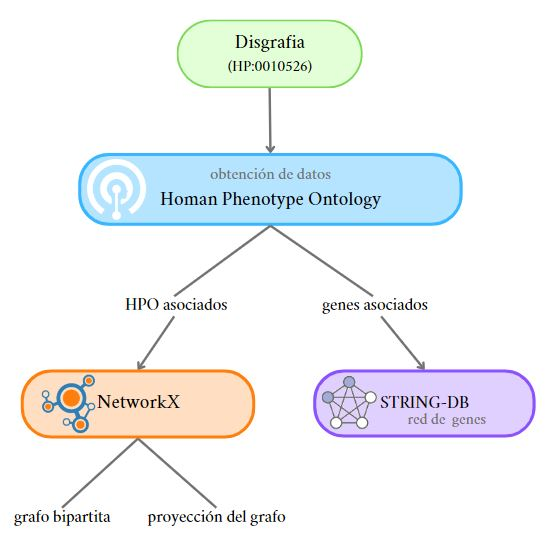
\includegraphics[width=0.7\textwidth]{figures/workflow.JPG}
	\caption{Flujo de trabajo}
	\label{fig:workflow}
\end{figure}

\subsection{Datos biológicos}

Lo primero que se realizó fue descargar los dataset necesarios para hacer el estudio. Se usaron dos base de datos: Human Phenotype Ontology (HPO) \cite{HPO2021} y STRING-DB \cite{String2021}.

\begin{enumerate}
	\item Se buscó el fenotipo Disgrafía en la HPO, conociendo que su identificador es HP:0010526. De esta base de datos, obtuvimos dos archivos tabulados; uno contiene los genes asociados y el otro contiene términos HPO asociados a la Disgrafía.
	\item La base de datos STRING se usó para descargar la red de interacción de proteínas humanas
\end{enumerate}


A continuación, se van a describir los distintos conjuntos de datos mencionados anteriormente.

\begin{itemize}
	\item \textbf{HPO asociados}
\end{itemize}

Uno de los archivos enumera para cada gen las clases HPO más específicas. Las primeras cinco filas se pueden visualizar en la tabla \ref{tabla:geneshpo}.

\renewcommand{\arraystretch}{1.5} % add more vertical space between cells in the table

\begin{table}[h!]
	\centering
	\caption{Cabecera del archivo de HPO asociados}
	\label{tabla:geneshpo}
	\resizebox{1.1\textwidth}{!}{
		\begin{tabular}{|c|c|c|c|c|c|c|}
			\hline
			Gene id (ncbi) & Gene symbol & HPO id & HPO name & frequency & Disease id \\
			\hline
			10 & NAT2 & HP:0000007 & Autosomal recessive inheritance & - & OMIM:243400 \\
			10 & NAT2 & HP:0001939 & Abnormality of metabolism/homeostasis & - & OMIM:243400 \\
			16 & AARS1 & HP:0002460 & Distal muscle weakness & 15/15 & OMIM:613287 \\
			16 & AARS1 & HP:0002451 & Limb dystonia & 3/3 & OMIM:616339 \\
			16 & AARS1 & HP:0008619 & Bilateral sensorineural hearing impairment & HP:0040283 & ORPHA:33364 \\
			\hline
		\end{tabular}
	}
\end{table}

La tabla \ref{tabla:geneshpo} proporciona el identificador de gen NCBI, el símbolo del gen, el identificador HPO y el nombre del término. Si está disponible, se muestra la frecuencia. Para este campo, hay tres opciones:

\begin{enumerate}
	\item Un identificador de término dentro de la sub-ontología de la HPO que esté relacionado con la frecuencia del fenotipo en cuestión
	\item Un recuento de pacientes afectados dentro de un individuo. "7/13" indicaría que 7 de los 13 pacientes con la enfermedad especificada tienen la anormalidad fenotípica mencionada por el término de la HPO en cuestión. Por ejemplo, la mutación en el gen AARS1 causa \textit{leucoencefalopatía}. La frecuencia del término HPO Ataxia sensorial esta anotada como 1 de 2 debido a la información en Sundal C, et al. \cite{Sundal2019}. 
	\item Un valor porcentual. Nuevamente, esto se refiere al porcentaje de pacientes que tienen la anormalidad fenotípica mencionada por el término de la HPO.
\end{enumerate}

La última columna muestra anotaciones realizadas por el equipo HPO (utilizando identificadores de enfermedades de OMIM), así como anotaciones proporcionadas por el equipo de Orphanet \cite{Orphanet2008} (utilizando identificadores de enfermedades de ORPHA).

El archivo se introdujo en Python como un data frame utilizando la librería Pandas \cite{pandasPython}. A través de operaciones lógicas aplicadas al data frame, se intentó inferir la existencia de algún gen que estuviera exclusivamente relacionado con la Disgrafía, sin tener asociación con otro término HPO.

\begin{itemize}
	\item \textbf{Genes asociados}
	\label{section:genesAsociados}
\end{itemize}

El segundo archivo consiste en un listado de genes asociados a la disgrafía. En la tabla \ref{tabla:genesAsociados}, se presenta la cabecera del archivo, donde también se visualizan tres columnas: la primera contiene el identificador de Entrez de los genes, la segunda el símbolo de los genes y la tercera el identificador de las enfermedades. Al igual que en el archivo anterior, el identificador de las enfermedades puede provenir de dos fuentes, OMIM o Orphanet.

\begin{table}[h]
	\centering
	\caption{Cabecera del archivo de genes asociados}
	\label{tabla:genesAsociados}    
	\resizebox{\textwidth}{!}{
		\begin{tabular}{|c|c|c|}
			\hline
			Gene id (entrez) & Gene symbol & DISEASE\_IDS \\
			\hline
			10347 & ABCA7 & ORPHA:1020,OMIM:608907 \\
			351 & APP & OMIM:605714,ORPHA:100006,ORPHA:1020,ORPHA:3247... \\
			9031 & BAZ1B & ORPHA:904 \\
			9275 & BCL7B & ORPHA:904 \\
			657 & BMPR1A & OMIM:174900,ORPHA:329971,OMIM:610069,ORPHA:157... \\
			\hline
		\end{tabular}
	}
\end{table}

\begin{itemize}
	\item \textbf{Red proteínas}
\end{itemize}

Este archivo contiene una red de interacciones entre proteínas humanas, presentes en la base de datos STRING, junto con una puntuación de los enlaces entre las proteínas. La cabecera de este archivo se puede visualizar en la tabla \ref{tabla:redProteinas}.

%\newcolumntype{C}{>{\centering\arraybackslash} p{4.5cm} }

\begin{table}[h]
	\centering
	\caption{Datos de la red de proteínas con puntuaciones combinadas.}
	\label{tabla:redProteinas} 
	\begin{tabular}{|c|c|c|}
		\hline
		\textbf{Proteína 1} & \textbf{Proteína 2} & \textbf{Puntuación Combinada} \\
		\hline
		9606.ENSP00000000233 & 9606.ENSP00000356607 & 173 \\
		9606.ENSP00000000233 & 9606.ENSP00000427567 & 154 \\
		9606.ENSP00000000233 & 9606.ENSP00000253413 & 151 \\
		9606.ENSP00000000233 & 9606.ENSP00000493357 & 471 \\
		\hline
	\end{tabular}
\end{table}

Cada fila contiene el StringID de las dos proteínas que interactúan, junto con el \textit{combined score}. Esta puntuación se calcula al combinar las probabilidades de diferentes canales de evidencia y se corrige por la probabilidad de observar una interacción al azar.

Este archivo es demasiado grande para subirlo al repositorio, por lo que se ha filtrado por el \textit{combined score} utilizando expresiones regulares:

\begin{verbatim}
	awk -F" " '$3 > 800 {print $0}'
	9606.protein.links.v12.0.txt > proteinas_filtrado.txt
\end{verbatim}

De esta forma, nos quedamos con aquellas interacciones que tengan una puntuación mayor a 800.

\subsection{Grafo bipartito}

Al no encontrarse ningún gen que afecte solo a Disgrafía, se buscó aquellos términos HPO relacionados [...]

En un grafo bipartito, los vértices se organizan en dos conjuntos distintos, de modo que cada arista conecta un vértice de un conjunto con otro del segundo conjunto. En términos más simples, no existen aristas que conecten vértices dentro del mismo conjunto \cite{BiRank2017}. En nuestro contexto, los conjuntos de vértices representan genes y términos HPO. De esta manera, obtenemos un grafo bipartito que conecta distintos términos HPO al nuestro, a través de genes. 

Para llevar a cabo esta representación y conexión entre genes y términos HPO, hemos utilizado la librería de Python NetworkX \cite{BookNetworkX}. Usando las segunda y tercera columna de la tabla \ref{tabla:geneshpo}, es decir los símbolos de los genes y los identificadores de los términos HPO, se creó este grafo bipartito. [...]

De este grafo nos interesaba ver aquellos término HPO que se encuentran estrechamente relacionados con la Disgrafía, por lo que lo siguiente que hicimos fue hacer un subgrafo que con los nodos que se encuentre a dos pasos del término HPO Disgrafía y hacer una proyección de los términos HPO de ese subgrafo. De esta forma obtuvimos aquellos HPO que están relacionados con al Disgrafía a través de un gen. [...].

\subsection{Red de genes}

A continuación, se procedió a realizar un estudio de los genes relacionados con la disgrafía (usando el archivo descrito en \ref{section:genesAsociados}). Lo primero fue obtener la red de genes utilizando la API de String-DB \cite{String2021}, haciendo uso de la biblioteca \textit{strindb} para Python. Entre las funciones clave de esta biblioteca se encuentra get\_network, la cual requiere como parámetros la lista de nuestros genes y el identificador de la especie \textit{Homo sapiens} (9606). Adicionalmente, se ha impuesto un score de 500, esta es una puntuación de corte para los bordes de la red, corresponde a la probabilidad de pertenecer a la misma vía funcional, lo que se traduce en que salgan más o menos genes en nuestra red.

La función devuelve la red de genes, donde se encuentran representados los genes y las relaciones entre ellos, la cual guardamos en un archivo .tsv.


\subsection{Propagación de la red}

Una vez que tenemos la red con los genes asociados, llevamos a cabo una propagación de la red con el objetivo de ampliar su tamaño y buscar otros genes relacionados con la Disgrafía. Este enfoque nos permite potencialmente descubrir otros genes implicados en la Disgrafía.

Para llevar a cabo este proceso, existen diferentes algoritmos, entre los cuales hemos seleccionado Diamond \cite{Diamond2015}.

Este algoritmo toma como parámetros nuestra red de genes, la red de interacciones de proteínas (filtrada), el número de genes que queremos que tenga el grafo final, y el nombre del archivo donde se va a guardar la red ampliada.

\begin{verbatim}
	python DIAMOnD.py proteinas_filtrado.txt grafo_51_genes.txt 200
	propaged_genes.txt
\end{verbatim}

\subsection{Detección de comunidades}

Para estudiar el grafo ampliado y la relación de los nuevos genes añadidos con el HPO de interés, se ha llevado a cabo un análisis de comunidades.

La detección de comunidades consiste en fragmentar el grafo en conjuntos de nodos, denominados "comunidades", teniendo en cuenta la topología de la red. En resumen, puede conceptualizarse como un proceso de agrupamiento (clustering) aplicado a grafos. Aunque no hay una definición única de comunidad aceptada por la comunidad científica, generalmente se considera que una comunidad es de calidad cuando muestra más conexiones internas que externas. En otras palabras, los nodos dentro de la comunidad están más densamente conectados entre sí en comparación con los nodos fuera de la comunidad en el grafo \cite{PanizoLledot}.

Para hacer la detecciónn de comunidades del grafo se ha usado uno de los algortimos proporcionados por el paquete NetworkX,\textit{ greedy\_modularity\_communities}. Este algoritmo utiliza la maximización de modularidad avariciosa de Clauset-Newman-Moore \cite{Clauset2004} para encontrar la partición de comunidades con la mayor modularidad.


\subsection{Enriquecimiento funcional}

El análisis funcional de genes implica registrar y analizar estadísticamente listas de genes con el objetivo de identificar anotaciones funcionales en relación con los genes analizados. El propósito principal es determinar si existe una asociación significativa entre los genes y las funciones específicas que desempeñan en procesos biológicos, rutas metabólicas u otras categorías funcionales. 

El enriquecimiento funcional se ha llevado a cabo utilizando el paquete String de Python, específicamente la función \textit{get\_enrichment}. Este análisis se ha realizado en varias ocasiones: una vez para el grafo ampliado y otra para cada una de las comunidades detectadas en la sección anterior.
	\section{Resultados}

En esta sección se van a presentar los resultados obtenidos tras realizar el estudio del fenotipo Disgrafía.

\subsection{Grafo bipartito}

Se ha observado, gracias al grafo proyectado de genes, que la disgrafía se relaciona con todos los 51 del archivo del que se obtuvo el grafo y (por medio de dichos genes) a 1357 términos HPO distintos. Como resultados del grafo bipartito se ha obtenido una tabla con las relaciones de cada uno de los HPOs acompañados por su nombre e identificador, ordenados según el número de genes que relacionen ese HPO con el de la disgrafía. En la tabla \ref{tab:dysgraphia-relaciones} se visualiza los HPO más realcionados con Disgrafía.

\begin{table}[h]
	\caption{HPO más relacionados con dysgraphia.}
	\label{tab:dysgraphia-relaciones}
	\centering
	\begin{tabular}{|c|c|c|}
		\hline
		\textbf{id HPO} & \textbf{Nombre} & \textbf{nº de genes} \\
		\hline
		HP:0010526 & Dysgraphia & 51 \\
		HP:0001288 & Gait disturbance & 45 \\
		HP:0000716 & Depression & 44 \\
		HP:0001260 & Dysarthria & 42 \\
		HP:0000739 & Anxiety & 42 \\
		HP:0002167 & Abnormality of speech or vocalization & 40 \\
		HP:0002017 & Nausea and vomiting & 38 \\
		HP:0001249 & Intellectual disability & 36 \\
		HP:0000505 & Visual impairment & 35 \\
		HP:0007018 & Attention deficit hyperactivity disorder & 35 \\
		\hline
	\end{tabular}

\end{table}


\subsection{Red de genes asociados}

Después de descargar la red de genes asociados a la Disgrafía de la HPO, observamos que contenía 51 genes. Posteriormente, obtuvimos la red de esos genes utilizando la base de datos STRING-DB, la cual se puede observar en la imagen \ref{fig:genesAsociados}.

\begin{figure}[h!]
	\centering
	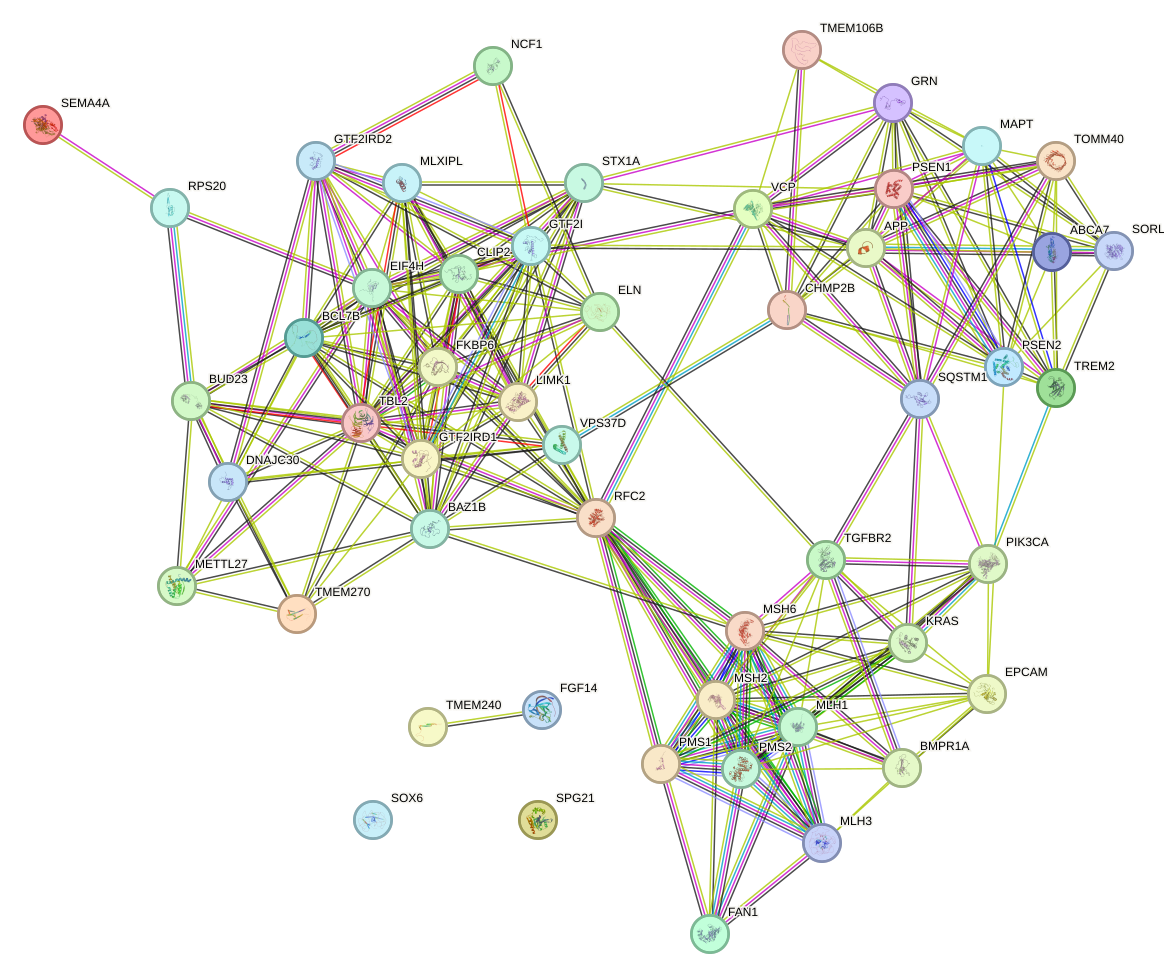
\includegraphics[width=0.7\textwidth]{figures/stringdb_51_genes.png}
	\caption{Red de genes asociados}
	\label{fig:genesAsociados}
\end{figure}

Se aplicó el algoritmo Diamond para propagar la red de genes y descubrir potenciales genes adicionales relacionados con la Disgrafía. El resultado de este proceso se encuentra en el archivo "propaged\_genes.txt", que contiene un listado con 200 genes. Utilizando estos genes, se creó una red mediante la librería de String. La cabecera del archivo que contiene la red se puede visualizar en la tabla \ref{tabla:resultDiamond} (se han omitido algunas columnas del archivo para mejor visualización).

\begin{table}[h]
	\centering
	\caption{Red de genes con los resultados de Diamond}
	\label{tabla:resultDiamond}
	\begin{tabular}{|c|c|c|c|c|c|}
		\hline
		stringId\_A & stringId\_B & preferredName\_A & preferredName\_B & score \\
		\hline
		9606.ENSP00000013807 & 9606.ENSP00000265433 & ERCC1 & NBN & 0.7 \\
		9606.ENSP00000013807 & 9606.ENSP00000347232 & ERCC1 & BLM & 0.701 \\
		9606.ENSP00000013807 & 9606.ENSP00000494957 & ERCC1 & UBE2T & 0.702 \\
		9606.ENSP00000013807 & 9606.ENSP00000229769 & ERCC1 & FANCE & 0.71 \\
		\hline
	\end{tabular}
\end{table}

Cada fila de esta red contiene información sobre la interacción de dos proteínas. Las cuatro primeras columnas incluyen los identificadores de los dos genes que están interactuando (tanto el StringId como el nombre). La cuarta columna (\textit{score}) es la puntuación combinada, la cual ya se mencionó en la sección \ref{section:redProteinas}.


\subsection{Detección de comunidades}

Se realizó un análisis de detección de comunidades en la red ampliada de genes. El algoritmo greedy\_modularity\_communities de NetworkX se empleó para identificar conjuntos de genes más densamente conectados entre sí. Los resultados de este análisis se presentan en la imagen \ref{fig:comunidades}.

\begin{figure}[h!]
	\centering
	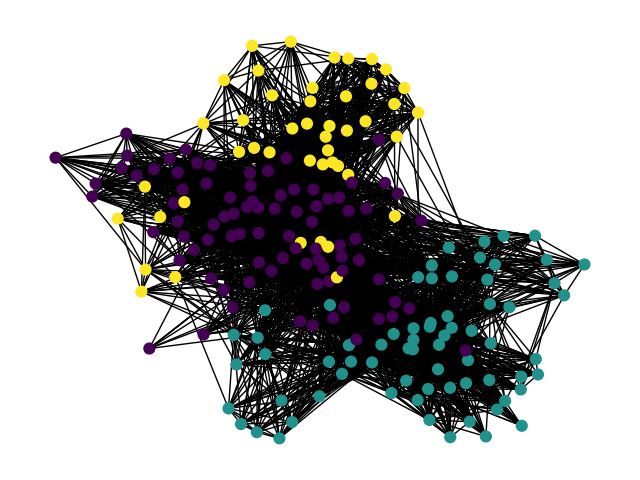
\includegraphics[width=0.7\textwidth]{../results/graph_communities.png}
	\caption{Comunidades de la red de genes}
	\label{fig:comunidades}
\end{figure}

Este algoritmo ha detectado tres comunidades. Cada color de la imagen \ref{fig:comunidades} representa una comunidad distinta.

\subsection{Enriquecimiento}

Se llevó a cabo un análisis de enriquecimiento funcional para identificar asociaciones significativas entre los genes y funciones específicas en procesos biológicos y rutas metabólicas. Este análisis se realizó tanto en el grafo ampliado como en cada una de las comunidades detectadas en la red de genes. La cabecera de los resultados se muestran en tablas \ref{tabla:enrique200}, \ref{tabla:enrique1}, \ref{tabla:enrique2} y \ref{tabla:enrique4}.

Cada conjunto de resultados del enriquecimiento ha sido ordenado de manera ascendente según el false discovery rate (FDR).


\begin{table}[h]
	\centering
	\caption{Enriquecimiento grafo ampliado}
	\label{tabla:enrique200}
	\begin{tabular}{|c|c|c|c|c|}
		\hline
		category & number\_of\_genes & p\_value & fdr & description \\
		\hline
		Process & 181 & $4.35 \times 10^{-220}$ & $6.83 \times 10^{-216}$ & DNA metabolic process \\
		Process & 150 & $1.01 \times 10^{-184}$ & $7.94 \times 10^{-181}$ & DNA repair \\
		Process & 158 & $2.57 \times 10^{-176}$ & $1.34 \times 10^{-172}$ & Cellular response to DNA damage stimulus \\
		Process & 189 & $1.61 \times 10^{-160}$ & $6.32 \times 10^{-157}$ & Nucleic acid metabolic process \\
		RCTM & 122 & $2.07 \times 10^{-155}$ & $4.72 \times 10^{-152}$ & DNA Repair \\

		Keyword & 123 & $2.2 \times 10^{-147}$ & $1.48 \times 10^{-144}$ & DNA damage \\
		Process & 185 & $1.9 \times 10^{-142}$ & $4.96 \times 10^{-139}$ & Cellular macromolecule metabolic process \\
		\hline
	\end{tabular}
\end{table}


\begin{table}[h]
	\centering
	\caption{Enriquecimiento primera comunidad}
	\label{tabla:enrique1}
	\begin{tabular}{|c|c|c|c|c|}
		\hline
		category & number\_of\_genes & p\_value & fdr & description \\
		\hline
		NetworkNeighborAL & 67 & $3.19 \times 10^{-123}$ & $1.46 \times 10^{-119}$ & DNA repair pathways, full network,...\\
		NetworkNeighborAL & 63 & $2.43 \times 10^{-117}$ & $3.71 \times 10^{-114}$ & Mixed, incl. Fanconi anemia pathway, ... \\
		NetworkNeighborAL & 64 & $4.23 \times 10^{-117}$ & $4.84 \times 10^{-114}$ & DNA repair pathways, ...\\
		Process & 85 & $8.09 \times 10^{-118}$ & $1.27 \times 10^{-113}$ & DNA metabolic process \\
		Process & 79 & $7.43 \times 10^{-116}$ & $5.83 \times 10^{-112}$ & DNA repair \\
		RCTM & 72 & $2.01 \times 10^{-112}$ & $4.6 \times 10^{-109}$ & DNA Repair \\
		NetworkNeighborAL & 60 & $2.65 \times 10^{-111}$ & $2.43 \times 10^{-108}$ & DNA repair pathways, full network, ... \\
		\hline
	\end{tabular}
\end{table}

\begin{table}[h]
	\centering
	\caption{Enriquecimiento segunda comunidad}
	\label{tabla:enrique2}
	\begin{tabular}{|c|c|c|c|c|}
		\hline
		category & number\_of\_genes & p\_value & fdr & description \\
		\hline
		NetworkNeighborAL & 43 & $1.52 \times 10^{-84}$ & $6.96 \times 10^{-81}$ & DNA replication, and Regulation ... \\
		Process & 47 & $3.04 \times 10^{-74}$ & $4.77 \times 10^{-70}$ & DNA replication \\
		RCTM & 43 & $8.24 \times 10^{-71}$ & $1.88 \times 10^{-67}$ & Mitotic G1 phase and G1/S transition \\
		RCTM & 41 & $2.06 \times 10^{-68}$ & $2.35 \times 10^{-65}$ & G1/S Transition \\
		RCTM & 42 & $3.76 \times 10^{-67}$ & $2.86 \times 10^{-64}$ & S Phase \\
		Process & 41 & $1.32 \times 10^{-67}$ & $1.03 \times 10^{-63}$ & DNA-templated DNA replication \\
		\hline
	\end{tabular}
\end{table}

\begin{table}[h]
	\centering
	\caption{Enriquecimiento tercera comunidad}
	\label{tabla:enrique4}
	\begin{tabular}{|c|c|c|c|c|}
		\hline
		category & number\_of\_genes & p\_value & fdr & description \\
		\hline
		Keyword & 41 & $1.25 \times 10^{-66}$ & $8.42 \times 10^{-64}$ & DNA repair \\
		WikiPathways & 34 & $1.55 \times 10^{-63}$ & $1.21 \times 10^{-60}$ & DNA repair pathways, full network \\
		Process & 43 & $1.62 \times 10^{-64}$ & $2.55 \times 10^{-60}$ & DNA repair \\
		NetworkNeighborAL & 35 & $1.43 \times 10^{-62}$ & $6.52 \times 10^{-59}$ & DNA repair pathways, full network, ... \\
		RCTM & 37 & $1.56 \times 10^{-57}$ & $3.55 \times 10^{-54}$ & DNA Repair \\
		COMPARTMENTS & 25 & $7.26 \times 10^{-50}$ & $1.67 \times 10^{-46}$ & DNA repair complex \\
		Component & 24 & $3.74 \times 10^{-49}$ & $7.66 \times 10^{-46}$ & DNA repair complex \\
		PMID & 30 & $1.19 \times 10^{-51}$ & $5.2 \times 10^{-45}$ & (2012) Exonuclease 1 (EXO1) ...\\
		\hline
	\end{tabular}
\end{table}


\clearpage
	\section{Discusión}

Tras observar los genes con los que se relacionan y las comunidades que forman (tabla \ref{tabla:enrique200}), resalta que la mayoría de ellos participan en actividades relacionadas con la reparación, formación y procesos metabólicos del ADN.\\

Además, si nos fijamos en estudios previamente realizados en torno a comunidades compuestas por los genes en cuestión, se desarrollan en este mismo contexto de reparación genómico. El artículo de Mota, M.B.S. et al. \cite{Mota2019} relaciona genes que aparecen en nuestro grafo, como H2AX, TP53BP1, RAD51 y EXO1, con la reparación de roturas de doble cadena, que es una de las principales vías de reparación.\\


Por otro lado, los HPOs mayoritariamente relacionados con la disgrafía también forman parte de trastornos mentales o psicológicos como la depresión, ansiedad o problemas en la sincronización de la marcha (tabla \ref{tab:dysgraphia-relaciones}). De esta manera podemos centralizar que efectivamente es una afección cerebral y no motora muscular.\\

Sin embargo, lo anteriormente explicado no implica un gran descubrimiento acerca de este fenotipo, las primeras relaciones obtenidas en el estudio resultan ser ya conocidas u obvias. Es por ello que investigando más profundamente y buscando patrones comunes en los archivos de enriquecimiento, hemos encontrado dos relaciones comunes menos intuitivas y por tanto más significativas.\\

Como se ha mencionado anteriormente, muchos de los genes relacionados con disgrafía se encargan de la reparacion del ADN. Estos genes desempeñan un papel importante en el mantenimiento de la integridad genómica y en la protección contra el desarrollo del cáncer. Cuando la primera etapa de eliminar el zonas dañadas en el ADN es más activa que la última etapa de volver a sintetizar el ADN durante el proceso de reparación, este desequilibrio provoca una acumulación excesiva de productos intermedios de ADN sin reparar, lo cual a su vez aumenta el riesgo de mutaciones y cáncer. \cite{Song2012}.\\

Además, estudios relacionan la deficiencia en la reparación del daño al ADN nuclear con varios trastornos neurodegenerativos \cite{Jeppesen2011}. Gracias al enriquecimento del grafo ampliado podemos comprobar que la mayoría de los genes implicados en ese grafo se encuentran en el núcleo de la célula y se encargan de la reparación de daños.  Si los mecanismos de reparación del ADN no funcionan eficientemente, es más probable que se acumulen mutaciones y daños genéticos en las células, lo que podría contribuir al desarrollo de trastornos neurodegenerativos, como disgrafía\\

Fijando la categoría a 'TISSUES' en el enriquecimiento de los 200 genes, aparecen muchas entradas con descripción derivada del aparato reproductor femenino, así como el desarrollo embrionario: \textit{ Cervical carcinoma cell, Embryo, Female reproductive system, Uterus... }

\begin{table}[h]
	\centering
	\caption{Datos sobre la categoría 'TISSUES' en el enriquecimiento de los 200 genes.}
	\label{tab:datos-tissues}
	\begin{tabular}{|c|c|c|c|c|}
		\hline
		\textbf{Categoría} & \textbf{Nº de genes} & \textbf{p-value} & \textbf{FDR} & \textbf{Descripción} \\
		\hline
		TISSUES & 35 & 1.43e-24 & 3.47e-21 & Cervical carcinoma cell \\
		TISSUES & 48 & 4.1e-18 & 4.97e-15 & Leukemia cell \\
		TISSUES & 31 & 2.34e-17 & 1.89e-14 & Lymphocytic leukemia cell \\
		TISSUES & 49 & 2.15e-16 & 1.3e-13 & Blood cancer cell \\
		TISSUES & 39 & 2.01e-15 & 9.74e-13 & Embryo \\
		TISSUES & 22 & 4.33e-15 & 1.75e-12 & Pronephros \\
		TISSUES & 22 & 1.83e-09 & 6.36e-07 & Bone marrow cancer cell \\
		TISSUES & 16 & 2.55e-09 & 7.73e-07 & Chronic lymphocytic leukemia cell \\
		TISSUES & 101 & 9.29e-09 & 2.5e-06 & Female reproductive system \\
		TISSUES & 56 & 1.43e-08 & 3.46e-06 & Organism form \\
		TISSUES & 5 & 2.36e-08 & 5.21e-06 & U2-OS cell \\
		TISSUES & 53 & 2.42e-08 & 5.21e-06 & Embryonic structure \\
		TISSUES & 103 & 3.74e-08 & 6.97e-06 & Reproductive system \\
		\hline
	\end{tabular}
	
\end{table}

Esta segmentación puede ser muy significativa dando pie a hipótesis sobre si el origen de la disgrafía está relacionada con el desarrollo embrionario o con la concepción. Además, se puede hilar a la alta interacción de estos genes con afecciones cancerígenas puesto que aparecen entradas sobre cáncer ovárico en el enriquecimiento \cite{Mad2014}.\\

En general, se han encontrado varias posibles relaciones de la disgrafía con otras patologías, fenotipos y tejidos. De esta manera logramos ampliar el conocimiento sobre este HPO y focalizar su área de efecto para proponer tratamientos parecidos a estas relaciones resultantes.


	\section{Conclusiones}

	
	
	%%%%%%%%%%%%%%%%%%%%%%%%%%%%%%%%%%%%%%%%%%%%%%
	%% OTRA INFORMACIÓN                         %%
	%%%%%%%%%%%%%%%%%%%%%%%%%%%%%%%%%%%%%%%%%%%%%%
	
	\begin{backmatter}
	
		\section*{Abreviaciones}%% if any
			SLD: dificultades específicas del aprendizaje
		
		\section*{Disponibilidad de datos y materiales}%% if any
			Enlace al repositorio de GithHub: \url{https://github.com/nmartinser/HPO_Dysgraphia}
		
		\section*{Contribución de los autores}
			Usando las iniciales que habéis definido al comienzo del documento, debeis indicar la contribución al proyecto en el estilo:Debéis indicar aquí un enlace a vuestro repositorio de github.
			J.E : Encargado del análisis de coexpresión con R, escritura de resultados; J.R.S : modelado de red con python y automatizado del código, escritura de métodos; ...
			OJO: que sea realista con los registros que hay en vuestros repositorios de github. 
		
		
		%%%%%%%%%%%%%%%%%%%%%%%%%%%%%%%%%%%%%%%%%%%%%%%%%%%%%%%%%%%%%%%%%%%%%%%%%%%%%%%%%%%%%%%%
		%% BIBLIOGRAFIA: no teneis que tocar nada, solo sustituir el archivo bibliography.bib %%
		%% por el que hayais generado vosotros                                                %%
		%%%%%%%%%%%%%%%%%%%%%%%%%%%%%%%%%%%%%%%%%%%%%%%%%%%%%%%%%%%%%%%%%%%%%%%%%%%%%%%%%%%%%%%%
		
		\bibliographystyle{bmc-mathphys} % Style BST file (bmc-mathphys, vancouver, spbasic).
		\bibliography{bibliography}      % Bibliography file (usually '*.bib' )
	
	\end{backmatter}
\end{document}
